\section{Evaluation}

In this section the application will be evaluated against its goal by both qualitative and quantitative means. The overarching goal of this project was to create a non-intrusive application that provides accurate real-time feedback on a lifter's squat form. The application is evaluated against this goal by examining each of the three key parts of the goal - its intrusiveness, speed, and accuracy.

\subsection{Intrusiveness}
The first of the three evaluation criteria is the application's intrusiveness. 

The application has no requirement for the user to wear any specialised equipment or markers in order to be tracked. The lifter simply follows their usual procedure in walking the weight out from the rack, squatting, then walking back to the rack to return the weight.

A small amount of set-up is required however, as the user must take their Android device into the gym and find a place to rest it so that it is stable with a clear view of the area in which they will be squatting. The user must also ensure that there is no movement in the background before they begin squatting, which can be difficult in a busy gym.

In summary, the intrusiveness of the application is in the set-up procedure, but there is none during the lift itself. From this it is fair to say that the application is non-intrusive, as once set-up is complete the application requires minimum interaction. The user does not even need to watch the screen as they squat due to the feedback being given verbally.

\subsection{Speed}

\subsubsection{Frame Rate}
A quantitative measure of the real-time nature of the application is its frame rate. Due to the way in which the application is implemented, with a separate thread processing frames to that which displays them on the screen, there are two independent frame rates that we can measure.

The first is that of the graphics thread, reading frames from the camera and displaying them on the screen. This frame rate remained level at a value of 15 frames per second, and provided a smooth video feed throughout the running of the application. This caps the maximum perceived frame rate to the user, as it is not possible to display frames at a faster rate.

The second is that of the processing thread. Measuring the rate at which the core algorithm provides frames to be displayed by the graphics thread. This frame rate fluctuated dramatically depending on the stage of the algorithm.

During the initial detection stage of the algorithm, the frame rate varied between 90 and 110 frames per second. This is due to the requirement of very little processing at this point.

The frame rate during the tracking and analysis stage of the algorithm is the most important, as this is where the algorithm is most resource intensive. During tracking, the frame rate was observed to vary between 22 and 28 frames per second. This is considerably faster than the limit of 15 frames per second, and shows that the algorithm developed in this project to track and analyse squats is easily capable of running in real-time.

\subsubsection{Feedback}
The application provides verbal feedback after each squat has been completed. This can be considered real-time as the user does not need to wait until they have finished their squats to receive feedback. This means that the user can adjust their technique during their set of squats according to the feedback given, allowing them to learn to squat safely and effectively.

\subsection{Accuracy}
Perhaps the most difficult requirement to measure is the accuracy of the application. Several approaches are taken in this section to attempt to evaluate the application's accuracy both qualitatively and quantitatively. Accuracy can be broken down into two categories - tracking accuracy and analysis accuracy.

\subsubsection{Tracking}

Much of the tracking accuracy is determined by the robustness of the background subtraction algorithm. The background subtraction algorithm is reasonably accurate, and in fixed lighting conditions performs very well, removing all of the surroundings and leaving the lifter's silhouette in place.

The algorithm taking the largest object in the foreground means that background movement that is isolated from the lifter does not have an effect on the subtraction. This can be seen in figure~\ref{fig:goodbackground}, as a man enters the view and the application continues to track as normal.

\begin{figure}[H]
    \centering
    \subfigure{
            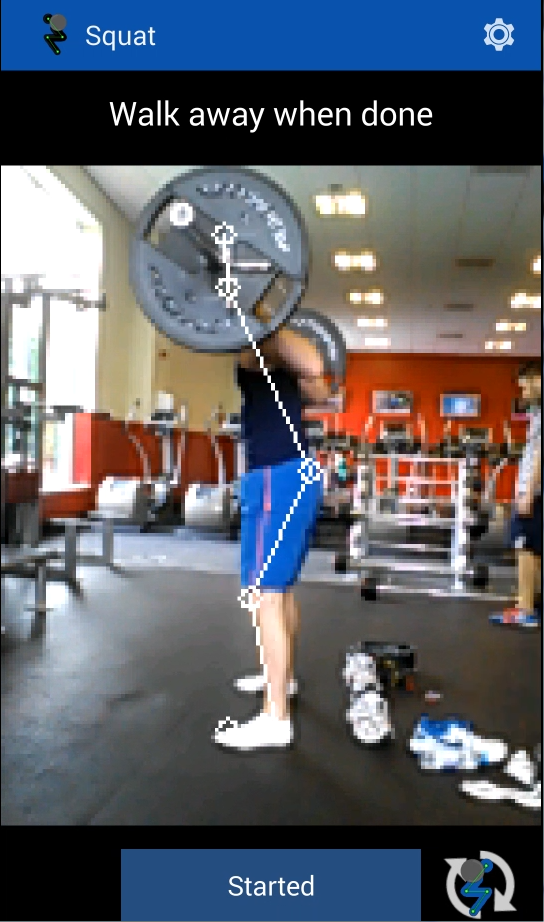
\includegraphics[height=7cm]{evaluation/images/goodbackground1}
    }
    \subfigure{
            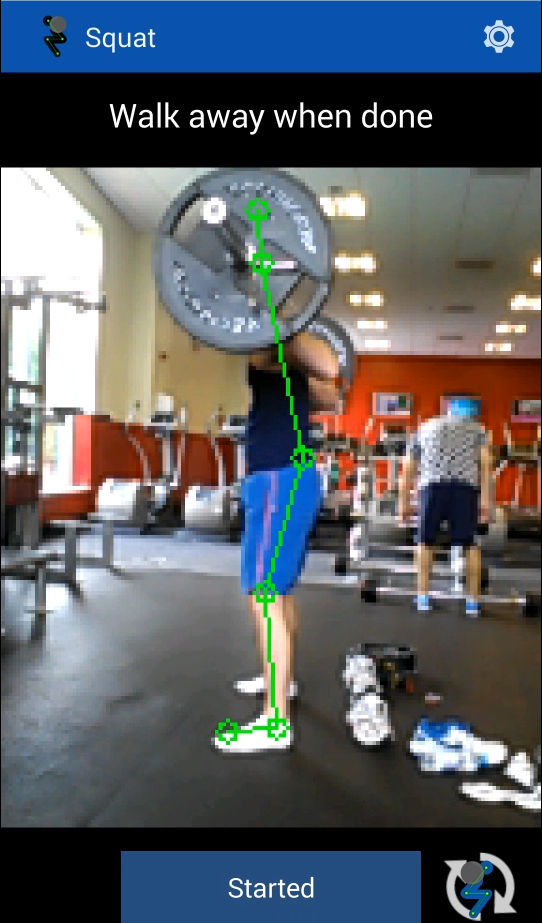
\includegraphics[height=7cm]{evaluation/images/goodbackground2}
    }
    \subfigure{
            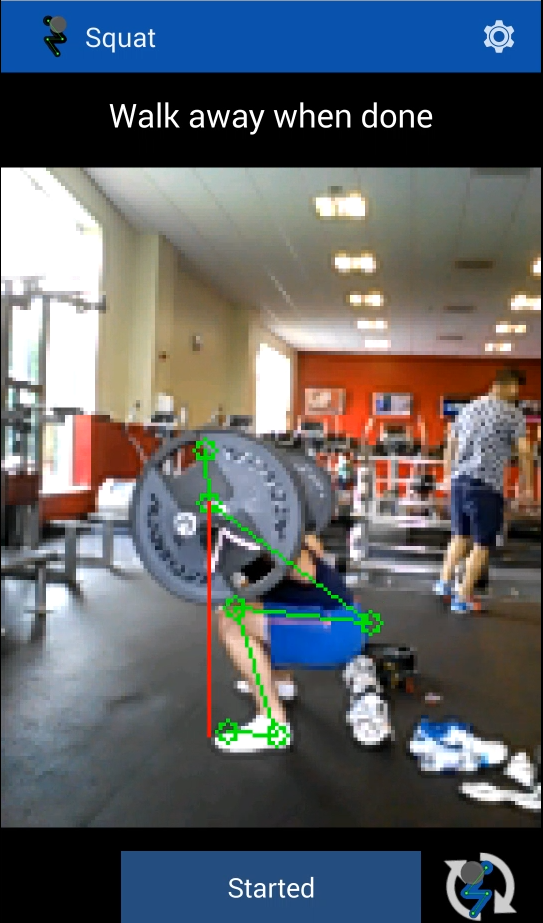
\includegraphics[height=7cm]{evaluation/images/goodbackground3}
    }
\caption{Isolated background movement does not affect tracking}
\label{fig:goodbackground}
\end{figure}

Any movement in the background or foreground that crosses the lifter will effect the subtraction however, as the largest object becomes the combination of the lifter and the disturbance. This can be seen in figure~\ref{fig:badtracking}.

\begin{figure}[H]
    \centering
    \subfigure{
            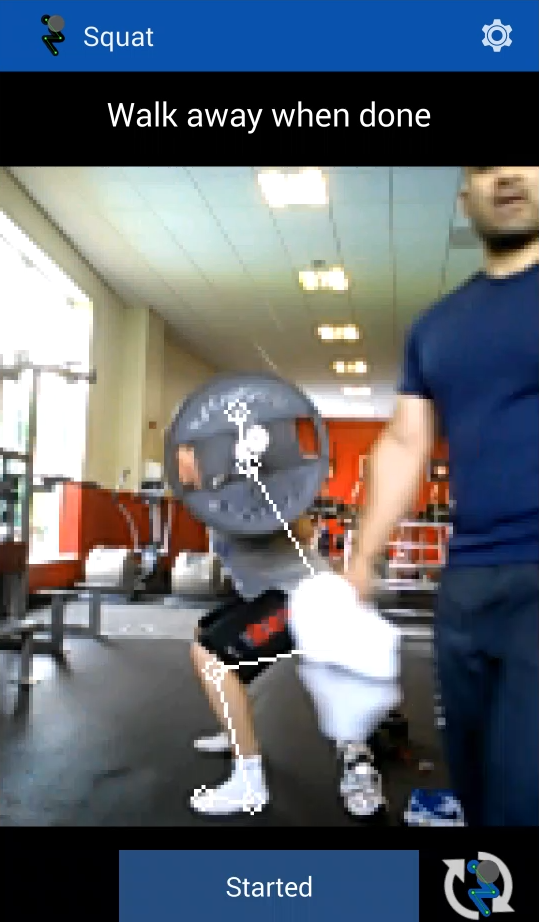
\includegraphics[height=7cm]{evaluation/images/badtracking1}
    }
    \subfigure{
            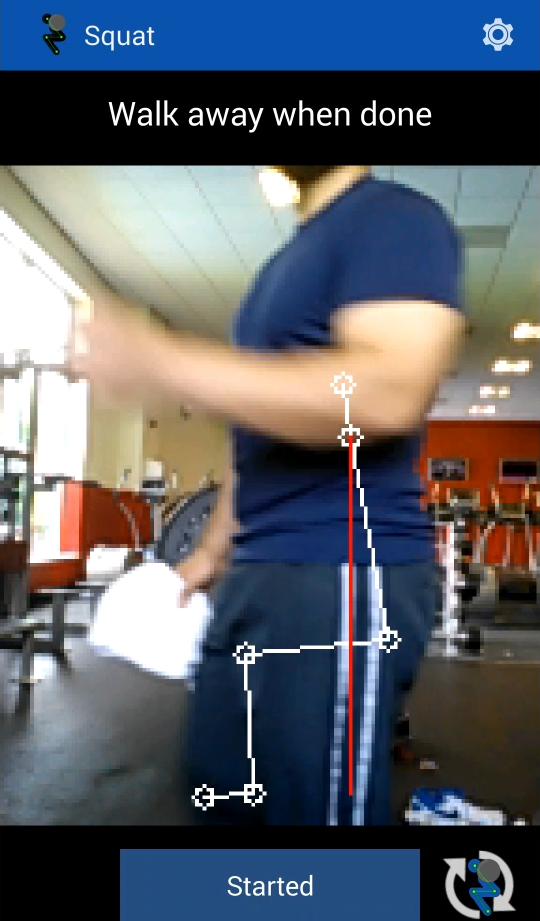
\includegraphics[height=7cm]{evaluation/images/badtracking2}
    }
    \subfigure{
            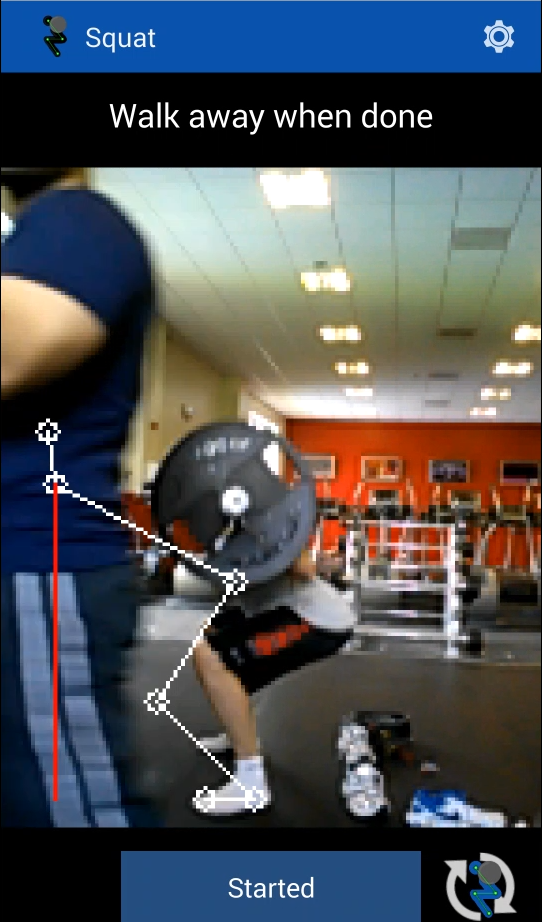
\includegraphics[height=7cm]{evaluation/images/badtracking3}
    }
\caption{A passer by upsets the tracking}
\label{fig:badtracking}
\end{figure}

As the passer by walks into view, he is detected as foreground, and as soon as he crosses the lifter, becomes part of the largest object, pulling the model towards him. The model follows the passer by until he leaves the view, but after this the model is reasonably quick to snap back into place and continue tracking the lifter as usual.

In poor lighting conditions, the background subtraction is prone to failure. When the lighting changes, the colour of pixels in the background will change and (as soon as the difference is greater than the threshold) will be detected as foreground. This then breaks down the tracking- wherever the model resides it achieves maximum overlap with the foreground.

\subsubsection{Analysis}

As the application analyses squat form using computer vision, it is difficult to evaluate it quantitatively. It is possible however to compare the scores given by the application with scores given by an expert observing the squat, to give a semi-quantitative measure of the application's performance.

%TODO lots of screenshots and tables and stuff from saturday's squat sesh!


\subsection{User Testing Evaluation}
In addition to the evaluation against the goal, the application was also evaluated by a set of users. These users took the application to the gym installed on a mobile device, and spent time using it to 


\begin{comment} % Comment out the eval plan stuff!!
\subsection{Goals}

My goals for this project are to have an easy to use application that will give real-time feedback on the execution of a squat and deadlift. The application should be non-intrusive, requiring no special equipment. It should be reasonably accurate, able to notify the lifter when they have executed a lift correctly or not.

\subsubsection{Squat Feedback}

The following feedback should be given to inform the user whether or not their squat was valid:

\begin{itemize}
	\item \textbf{Depth} Whether or not the hip joint goes below the knee at the bottom of the squat
	\item \textbf{Lockout} Whether or not the lifter fully locked out their knees and hips to finish in an upright position
	\item \textbf{Reverse Movement} Whether or not the lifter moved downwards in the ascent part of the squat
\end{itemize}

The following feedback should be given to inform the user whether or not their squat was safe:

\begin{itemize}
	\item \textbf{Upright Shins} Whether the shins remain near-vertical throughout the lift (to avoid knee injury)
	\item \textbf{Back Flexion} Whether the spine remained neutral during the lift (to avoid back injury)
	\item \textbf{Back Angle} Whether the back remains within an optimal range of angles during the lift
\end{itemize}

\subsection{Testing}

To test the core functionality of the app, I will provide a sample of gym-goers with a copy, and ask them to review it according to the following criteria:

\begin{itemize}
	\item Ease of Use
	\item Accuracy
	\item Effectiveness (ie. how much it helped their training)
\end{itemize}

To evaluate whether the application runs in real-time, I will benchmark test the frames per second of the application. A value above 10fps will be considered a suitable frame rate.

I will also test its accuracy by running the application against good and bad squats, and recording the number of true positives, false positives, true negatives and false negatives. These results will be used to give statistics on the success of the project.
\end{comment}